\documentclass{standalone}
\begin{document}
	\subsection{Pipeline Structure}
	
	In this section I will discuss the general structure of the pipeline, more details about the actual implementation will be given in the next chapter. As I've said before the pipeline is divided into two main phases, one for the centroids estimation, which is performed only once, and one of the actual segmentation, which is performed at least once for each scan to segment. Before each of these step we need also a preliminary step to achieve pre processing and a lung region isolation, useful to focus the segmentation in the region of interest and to avoid false positives.\\
	In the end the pipeline structure is divided in three main blocks as we can see in \figurename\,\ref{fig:Pipeline} : 
	\begin{itemize}
		\item \textbf{Pre-Processing and lung extraction}: Preliminary step, involves registration and isolation of lung regions;
		\item \textbf{Training} : involves the estimation of the centroids, is performed only ones; 
		\item \textbf{Labeling} : involves the assignement of each voxel to the cluster of the closest centroids, it is the actual segmentation.
	\end{itemize}
	
		
	\begin{figure}[h!]\label{fig:Pipeline}
		\centering 
		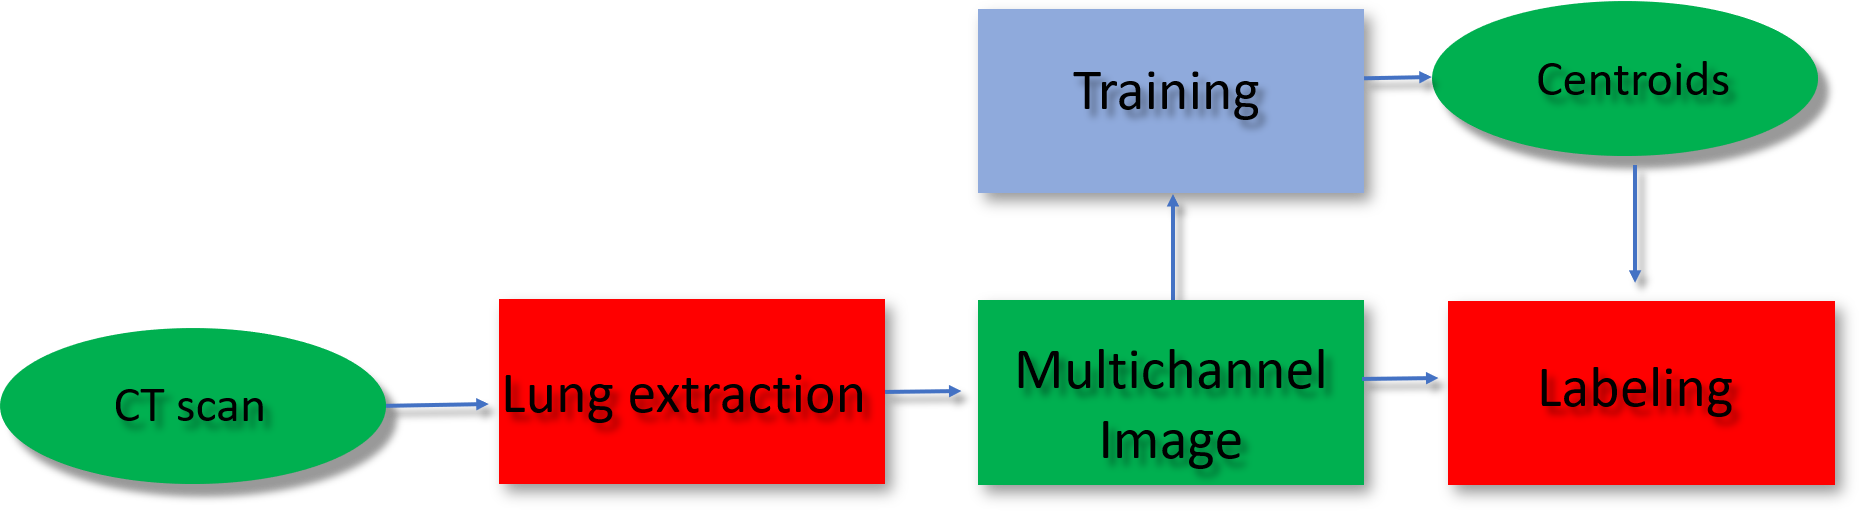
\includegraphics[width=.7\textwidth]{Pipeline.png}
		\caption{Flow chart of the main structure of the developed pipeline. The training process, which allows the estimation of the centroids, is perfromed only one time.}
	\end{figure} 
	
	
	\subsubsection*{Pre Processing and Lung Extraction}
	
	This preliminary step is performed before both training and labeling.\\
	First of all performs a registration of the HU on a common space, in order to overcomes the issues that may raise from the different padding values and multiplicative constant for HU computation(equation\,\ref{eq:HU}) used by the different manufacturer of the CT scans.\\
	This process is followed by a segmentation fo the lung regions, which allows to remove all the extra lung regions avoiding the formation of false positives. During this process a particular attention was paid on the removal of the main main bronchial structures, which can interfere with the actual segmentation, and the preservation of the lung regions which are the ones in which we are interested in.
	
	\subsubsection*{Training}
	
	This step involves the estimation of the centroids for each tissue. This step requires different patients, in order to have a good statistical representation of each structure, this the kmeans requires an homogeneous representation of each cluster. This makes the entire process time consuming and computational expansive,but, as I've said before, this process need to be performed only once, so isn't involved in the actual segmentation and doesn't affect the segmentation time.\\ The implementation of this step involves the building of the multichannel image, to takes into account the different features of the images like neighborhooding voxel intensity or edges, the managing of the over represented clusters like the background and the actual centroids estimation via kmeans clustering. All of these steps will be discuss in details in the next session.

	
	\subsection*{Labeling}
	
	This step involves the actual segmentation. The script which perform it requires as inputs the image after the lung extraction, and the previously estimated centroids. This block of the pipeline simply assign each voxel to the cluster corresponding to the nearest centroids and the end of the procedure only the cluster corresponding to the GGO are provided. In this way we are performing a pixel classification by assign regions to a particular labels according only to intensities information, without exploiting spatial information: this allow us to group on the same cluster objects that are spatially disconnected as often happen in medical imaging field. 
	To found the closest centroids we simply compute the euclidean distance between each voxel and each centroids and assign the vocxel to the closest cluster.
	
	In the end, once we have estimated the centroids, the segmentation pipeline will results of only two steps, as shown in \figurename\,\ref{fig:FinalPipeline} , in which we can observe the flowchart of each step with an image that shown the partial results.
	
	
	\begin{figure}\label{fig:FinalPipeline}
		\centering
			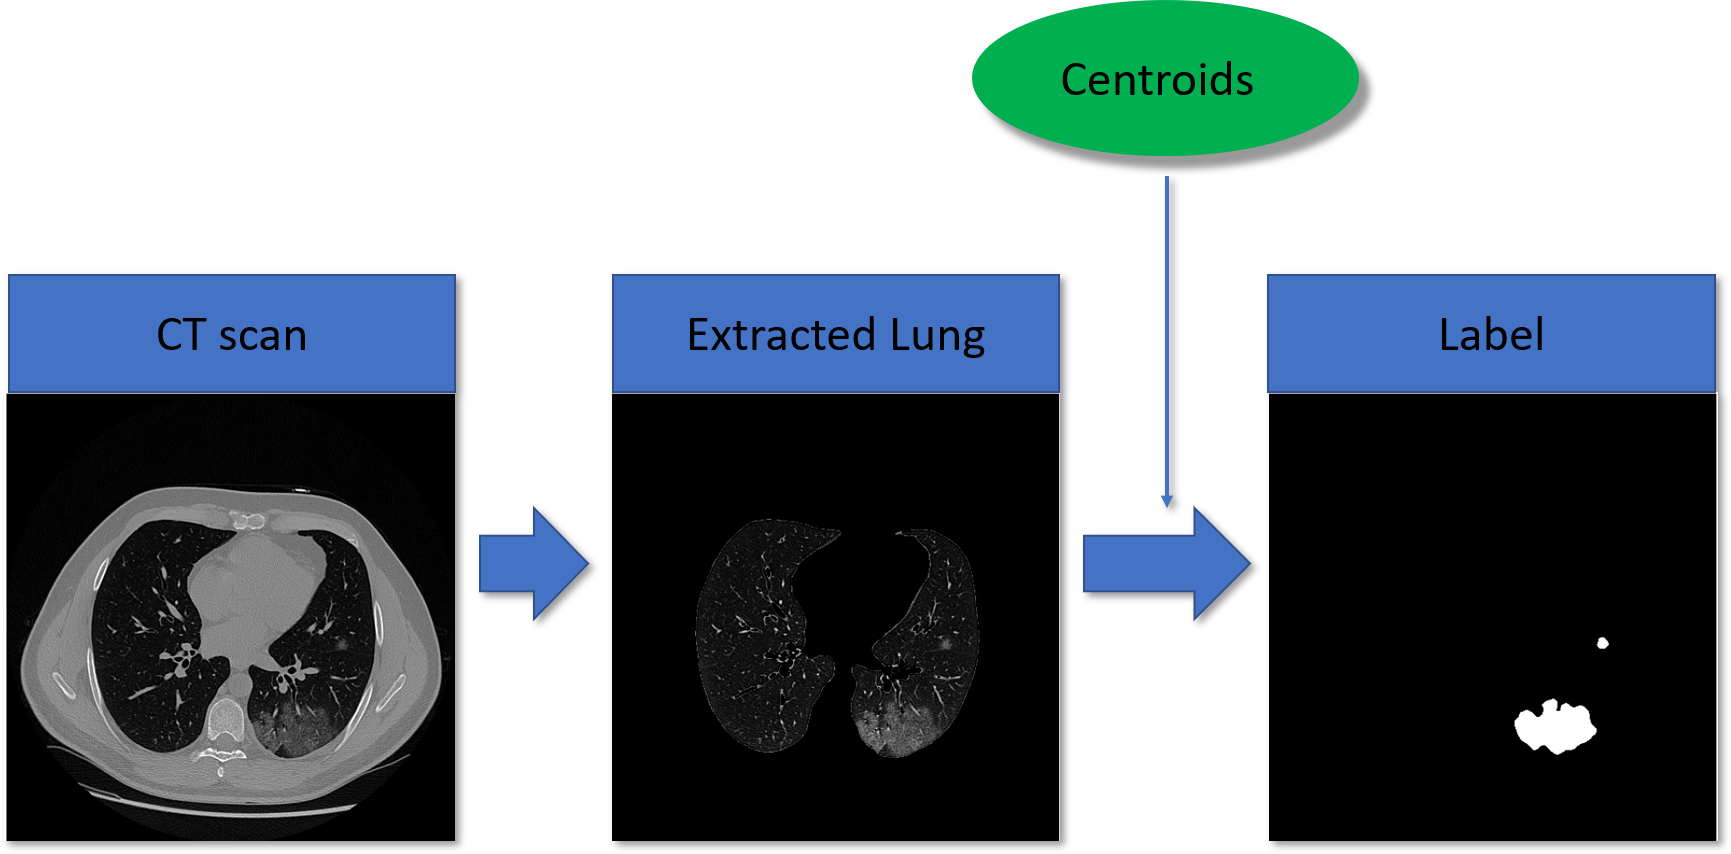
\includegraphics[width=.75\textwidth]{final_pipeline.png}
			\caption{Actual segmentation step, from left to right we can see the input image stack, the isolated lung regions and the final label. To performed the labeling a set of pre-computed centroids was used.}
	\end{figure}
	
	
	
\end{document}